\documentclass[12pt, a4paper]{article}

% --- PREAMBUŁA (ustawienia dokumentu) ---
\usepackage[utf8]{inputenc}       % Kodowanie znaków
\usepackage[T1]{fontenc}          % Polskie znaki (ą, ć, ę, ł, ń, ó, ś, ź, ż)
\usepackage[polish]{babel}        % Polskie reguły dzielenia wyrazów i nazwy (np. "Spis treści")
\usepackage{amsmath}              % Pakiety matematyczne (niezbędne do macierzy)
\usepackage{amsfonts}             % Czcionki matematyczne
\usepackage{amssymb}              % Symbole matematyczne (np. nieskończoność)
\usepackage{geometry}             % Ustawienia marginesów
\usepackage{csvsimple}
\usepackage{float}
\usepackage{graphicx}
\usepackage{siunitx}
\usepackage[utf8]{inputenc}
\usepackage[T1]{fontenc}
\usepackage{booktabs} % Wymagane przez pandas.to_latex()
\usepackage{textcomp} % Dla symbolu mikrona
\geometry{
	a4paper,
	left=2.5cm,
	right=2.5cm,
	top=2.5cm,
	bottom=2.5cm
}
\usepackage{indentfirst}          % Wcięcia w pierwszych akapitach
\usepackage{hyperref}             % Aktywne odnośniki w dokumencie
\usepackage{setspace}             % Interlinia
\setstretch{1.35}                 % ZWIĘKSZONA INTERLINIA (ok. 1.5 linii)
\setlength{\parskip}{0.5em}       % Dodatkowy odstęp między akapitami

% --- DANE DO STRONY TYTUŁOWEJ ---
\title{\textbf{Sprawozdanie z projektu nr 1} \\ \large Asymetryczny Problem Komiwojażera (ATSP)
\\ \large Projektowanie Efektywnych algorytmów}
\author{Karol Gąsior / 280913}
\date{\today} 

% --- POCZĄTEK WŁAŚCIWEGO DOKUMENTU ---
\begin{document}
	
	\maketitle % Generuje tytuł, autora i datę
	\newpage
	\tableofcontents % Automatyczny spis treści
	\newpage
	
	\section{Wstęp teoretyczny}
	
	\subsection{Sformułowanie problemu komiwojażera (TSP i ATSP)}
	Problem komiwojażera (ang. \textit{Traveling Salesperson Problem}, TSP) to jedno z najważniejszych zagadnień optymalizacji kombinatorycznej oraz informatyki teoretycznej. W swojej klasycznej postaci problem ten można sformułować następująco: dany jest zbiór $N$ miast oraz odległości pomiędzy każdą parą z nich. Celem jest znalezienie najkrótszej możliwej trasy, która rozpoczyna się w dowolnym mieście, odwiedza dokładnie raz każde z pozostałych miast i powraca do miasta początkowego.
	
	W ujęciu teorii grafów, problem modelowany jest za pomocą pełnego grafu ważonego $G = (V, E)$, gdzie $V$ to zbiór wierzchołków (miast) o mocy $|V| = N$, a $E$ to zbiór krawędzi (połączeń między miastami). Każdej krawędzi $(i, j) \in E$ przypisana jest waga (koszt) $c_{ij} \geq 0$. Szukanym rozwiązaniem jest cykl Hamiltona o minimalnej sumie wag krawędzi.
	
	W niniejszym projekcie rozpatrywany jest wariant asymetryczny problemu komiwojażera (ang. \textit{Asymmetric Traveling Salesperson Problem}, ATSP). Oznacza to, że graf $G$ jest grafem skierowanym, a macierz kosztów przejść nie musi być symetryczna, czyli w ogólnym przypadku zachodzi:
	$$ c_{ij} \neq c_{ji} \quad \text{dla} \quad i, j \in V $$
	Asymetria ta sprawia, że problem jest jeszcze trudniejszy do rozwiązania w optymalnym czasie. Ścieżka optymalna w jedną stronę może mieć zupełnie inny koszt (lub być wręcz niemożliwa ze względu na koszty dążące do nieskończoności) przy próbie jej odwrócenia. Problem ATSP należy do klasy problemów NP-trudnych, co oznacza, że nie jest znany żaden algorytm zdolny do znalezienia optymalnego rozwiązania w czasie wielomianowym dla każdego przypadku testowego.
	
	\subsection{Analiza i złożoność implementowanych algorytmów}
	W ramach prac projektowych zaimplementowano i zbadano cztery zróżnicowane podejścia algorytmiczne do problemu ATSP:
	
	\subsubsection{Przegląd zupełny (Brute-Force)}
	Algorytm przeglądu zupełnego to metoda dokładna, gwarantująca odnalezienie globalnego optimum. Jego działanie polega na wygenerowaniu przestrzeni wszystkich możliwych rozwiązań (cykli Hamiltona), obliczeniu funkcji celu (kosztu całkowitego) dla każdej z nich i wybraniu wartości minimalnej. 
	
	Z uwagi na fakt, że poszukiwany jest cykl, punkt startowy nie ma znaczenia dla ostatecznego kosztu całej trasy. Dlatego w zaimplementowanym algorytmie wierzchołek początkowy (miasto o indeksie $0$) jest na stałe ,,zamrożony'' na pierwszej pozycji. Pozwala to na zredukowanie liczby permutacji do wygenerowania z $N!$ do $(N-1)!$. 
	Całkowita złożoność obliczeniowa tego podejścia wynosi $O(N!)$. Złożoność silniowa rośnie w tak drastycznym tempie, że już dla stosunkowo niewielkich wartości $N$ (np. $N > 13$) czas potrzebny na wygenerowanie i sprawdzenie wszystkich tras przekracza możliwości współczesnych jednostek obliczeniowych w akceptowalnym czasie ludzkim.
	
	\subsubsection{Algorytm losowy (Random Search)}
	Algorytm losowy należy do grupy metod stochastycznych (probabilistycznych). Zamiast systematycznie przeszukiwać przestrzeń rozwiązań, algorytm ten w sposób ciągły losuje permutacje ścieżek i oblicza ich koszty, zachowując w pamięci tę, która do tej pory charakteryzowała się najmniejszą wagą sumaryczną. Nie jest to algorytm heurystyczny, gdyż nie wykorzystuje żadnej logiki problemu do kierowania swoimi decyzjami – opiera się wyłącznie na ślepym losowaniu przestrzeni.
	
	Pojedyncza iteracja (wylosowanie permutacji i obliczenie kosztu trasy o długości $N$) kosztuje asymptotycznie $O(N)$. Całkowita złożoność jest ściśle uzależniona od warunku stopu, którym w tym przypadku jest nałożony limit czasu. Choć algorytm ten wykonuje ogromną liczbę prób w jednostce czasu, prawdopodobieństwo losowego ,,trafienia'' w optymalną trasę przy dużej liczbie wierzchołków jest bliskie zeru. Algorytm ten często stanowi dolną granicę jakości (ang. \textit{baseline}) w ocenie pozostałych metod.
	
	\subsubsection{Najbliższy sąsiad (Nearest Neighbour - NN)}
	Jest to klasyczny algorytm zachłanny. Konstrukcja rozwiązania polega na wyborze wierzchołka startowego, a następnie, w każdym kolejnym kroku, dołączaniu do ścieżki tego spośród nieodwiedzonych wierzchołków, do którego koszt przejścia z obecnego węzła jest najmniejszy (lokalne optimum). 
	
	Decyzje podejmowane w każdym kroku są ostateczne (algorytm nie posiada mechanizmu nawrotów – ang. \textit{backtracking}). Z tego powodu algorytm NN często wpada w tzw. pułapki – zmuszony jest na samym końcu trasy do wybrania wyjątkowo kosztownych krawędzi zamykających cykl, co drastycznie pogarsza całkowity wynik.
	Złożoność obliczeniowa to $O(N^2)$, ponieważ dla każdego z $N$ miast algorytm musi przeszukać listę do $N-1$ potencjalnych sąsiadów. Jest to metoda skrajnie szybka, generująca rozwiązania natychmiastowo nawet dla bardzo dużych instancji problemu.
	
	\subsubsection{Powtarzalny najbliższy sąsiad (Repetitive Nearest Neighbour - RNN)}
	Jakość rozwiązania zwracanego przez zwykły algorytm NN jest silnie uzależniona od wyboru wierzchołka startowego – szczególnie w wariancie asymetrycznym macierzy. Aby zminimalizować to ryzyko, algorytm RNN uruchamia heurystykę Nearest Neighbour $N$ razy, za każdym razem inicjalizując trasę w innym wierzchołku. Po zebraniu $N$ różnych cykli, algorytm zwraca ten o najniższym koszcie. Złożoność czasowa wzrasta o jeden rząd wielkości do $O(N^3)$, co nadal plasuje go w kategorii algorytmów wielomianowych o bardzo wysokiej wydajności praktycznej.
	
	% ---------------------------------------------------------------------------------------------------------------------
	
	\section{Przykład praktyczny algorytmu Nearest Neighbour dla $N=3$}
	
	Dla lepszego zobrazowania mechaniki algorytmów zachłannych w przestrzeni asymetrycznej, przeanalizujmy działanie algorytmu Nearest Neighbour (NN) krok po kroku dla mikroskopijnej instancji problemu o rozmiarze $N=3$. Niech asymetryczna macierz kosztów przejść $M$ prezentuje się następująco:
	$$ M = \begin{bmatrix} \infty & 10 & 15 \\ 5 & \infty & 9 \\ 6 & 12 & \infty \end{bmatrix} $$
	Wartość $M[i][j]$ określa koszt jednokierunkowej podróży z miasta $i$ do miasta $j$. Na przekątnej znajdują się wartości $\infty$, uniemożliwiające podróż z danego miasta do niego samego.
	
	\textbf{Założenia początkowe:}
	Algorytm wymusza miasto startowe na indeksie $0$.
	
	\textbf{Krok 1: Stan początkowy}
	\begin{itemize}
		\item Aktualne miasto: $0$.
		\item Zbiór miast odwiedzonych: $V_{odwiedz} = \{0\}$.
		\item Zbiór miast nieodwiedzonych: $V_{nieodwiedz} = \{1, 2\}$.
		\item Aktualna ścieżka: $P = [0]$. Aktualny koszt całkowity: $C = 0$.
	\end{itemize}
	
	\textbf{Krok 2: Poszukiwanie pierwszego sąsiada}
	\begin{itemize}
		\item Z miasta $0$ algorytm skanuje krawędzie prowadzące do wierzchołków z $V_{nieodwiedz}$.
		\item Koszt podróży do miasta $1$: $M[0][1] = 10$.
		\item Koszt podróży do miasta $2$: $M[0][2] = 15$.
		\item Zgodnie z kryterium zachłannym, algorytm wybiera minimum lokalne: $\min(10, 15) = 10$. Wybrane zostaje miasto $1$.
		\item Aktualizacja stanu: $V_{odwiedz} = \{0, 1\}$, $V_{nieodwiedz} = \{2\}$.
		\item Aktualna ścieżka: $P = [0, 1]$. Aktualny koszt: $C = 0 + 10 = 10$.
	\end{itemize}
	
	\textbf{Krok 3: Poszukiwanie drugiego sąsiada}
	\begin{itemize}
		\item Z miasta $1$ pozostał tylko jeden wierzchołek do odwiedzenia: zbiór $V_{nieodwiedz}$ zawiera jedynie element $2$.
		\item Algorytm musi udać się do miasta $2$. Koszt podróży to: $M[1][2] = 9$.
		\item Aktualizacja stanu: $V_{odwiedz} = \{0, 1, 2\}$, zbiór miast nieodwiedzonych jest pusty.
		\item Aktualna ścieżka: $P = [0, 1, 2]$. Aktualny koszt: $C = 10 + 9 = 19$.
	\end{itemize}
	
	\textbf{Krok 4: Zamknięcie cyklu Hamiltona}
	\begin{itemize}
		\item Aby poprawnie rozwiązać problem komiwojażera, trasę należy zakończyć powrotem z ostatniego miasta do wierzchołka startowego.
		\item Koszt powrotu z miasta $2$ do miasta $0$ wynosi: $M[2][0] = 6$.
		\item \textbf{Ostateczna ścieżka:} $P_{final} = [0, 1, 2, 0]$.
		\item \textbf{Ostateczny koszt całkowity:} $C_{final} = 19 + 6 = 25$.
	\end{itemize}
	
	% ---------------------------------------------------------------------------------------------------------------------
	
	\section{Opis implementacji algorytmów i zastosowanych struktur}
	
	Całość projektu została zaimplementowana w języku C++ z rygorystycznym zachowaniem paradygmatu programowania obiektowego. Aby spełnić założenia optymalnego zarządzania pamięcią, zrezygnowano ze statycznych tablic wielowymiarowych. Używane struktury danych są alokowane w pełni dynamicznie na stercie w zależności od żądanego rozmiaru badanej instancji $N$.
	
	\subsection{Kluczowe struktury danych i mechanizmy pomocnicze}
	\begin{itemize}
		\item \textbf{Klasa \texttt{Array}:} Autorska, obiektowa reprezentacja asymetrycznej macierzy kosztów. Wewnątrz alokuje ciągły blok pamięci, co optymalizuje proces prefetchingu przez pamięć podręczną procesora i minimalizuje błędy braku w pamięci (ang. \textit{cache misses}) podczas gęstego odpytywania w algorytmach o wysokiej złożoności. Udostępnia metody dostępowe takie jak \texttt{get(row, col)}.
		\item \textbf{Klasa \texttt{Wektor}:} Dynamiczna tablica wskaźnikowa służąca do przechowywania permutacji miast (ścieżek) oraz flag odwiedzin w algorytmach zachłannych. Implementuje własne mechanizmy kopiowania (konstruktor kopiujący, operator przypisania) zapobiegające wyciekom pamięci.
		\item \textbf{Struktura \texttt{Result}:} Pełni rolę kontenera transportowego dla wyników działania każdego z algorytmów. Posiada pole \texttt{cost} reprezentujące minimalną znalezioną odległość oraz obiekt \texttt{path} (typu \texttt{Wektor}) przechowujący poprawną kolejność wierzchołków.
		\item \textbf{Zarządzanie czasem wykonania:} Wykorzystano wprowadzony w standardzie C++20 mechanizm \texttt{std::stop\_token}. Umożliwia on eleganckie i przede wszystkim w pełni bezpieczne z punktu widzenia wielowątkowości przerywanie działania nieskończonych pętli (jak w metodzie \texttt{tsp\_random}) lub pętli o potężnej liczbie iteracji (jak w metodzie \texttt{tsp\_brute\_force}) przez zewnętrzny kontroler czasu, eliminując potrzebę inwazyjnego odpytywania funkcji systemowych o aktualny czas wewnątrz najbardziej wrażliwych bloków obliczeniowych.
	\end{itemize}
	
	\subsection{Implementacja przeglądu zupełnego (Brute-Force)}
	Sercem algorytmu dokladnego jest funkcja \texttt{tsp\_brute\_force}. Pętla poszukująca optymalnego rozwiązania została oparta o konstrukcję \texttt{do-while}. Fundamentalnym problemem optymalizacyjnym jest tu generowanie permutacji. Zrezygnowano z bibliotecznej funkcji \texttt{std::next\_permutation} na rzecz implementacji własnej metody \texttt{nastepna\_permutacja} operującej na autorskiej klasie \texttt{Wektor}.
	
	Algorytm generowania permutacji opiera się na porządku leksykograficznym i składa się z następujących kroków:
	\begin{enumerate}
		\item Poszukiwanie od końca (od prawej do lewej) pierwszego takiego indeksu $i$, dla którego zachodzi $w[i] < w[i+1]$. Jeśli taki indeks nie istnieje, wygenerowano już wszystkie możliwe układy.
		\item Poszukiwanie od końca pierwszego indeksu $j$, dla którego $w[j] > w[i]$.
		\item Zamiana wartości pod indeksami $i$ oraz $j$ (\texttt{std::swap}).
		\item Odwrócenie kolejności elementów na prawo od indeksu $i$ (od $i+1$ do końca) za pomocą pomocniczej metody \texttt{odworoc\_wektor}.
	\end{enumerate}
	Co niezwykle istotne, implementacja ta ignoruje indeks $0$ wektora ścieżki. Złożoność $(N-1)!$ uzyskuje się poprzez zablokowanie pierwszego miasta i permutowanie zbioru wierzchołków od indeksu $1$ do $N-1$. 
	
	\subsection{Implementacja algorytmu losowego}
	Funkcja \texttt{tsp\_random} ma za zadanie działać nieprzerwanie aż do momentu zgłoszenia żądania zatrzymania przez \texttt{std::stop\_token}. Za generowanie pseudolosowości odpowiada wysoce wydajny generator Mersenne Twister (\texttt{std::mt19937}), inicjalizowany za pomocą ziarna pochodzącego z entropii sprzętowej systemu (\texttt{std::random\_device}).
	
	Do tasowania miast wykorzystano klasyczne generowanie porządku leksykalnego, zaimplementowany wewnątrz głównej pętli \texttt{while(true)}. Złożoność pojedynczego przetasowania wynosi $O(N)$. Po każdym przetasowaniu następuje ewaluacja wagi grafu i ewentualne nadpisanie struktury \texttt{out\_result}.
	
	\subsection{Implementacja algorytmów zachłannych (NN oraz RNN)}
	Główna logika Nearest Neighbour znajduje się w wydzielonej metodzie \texttt{tsp\_nn\_wew}. 
	Stan algorytmu śledzony jest przy użyciu wektora \texttt{visited}, zainicjowanego zerami. Algorytm wymusza $N-1$ kroków iteracyjnych. W każdym z nich wewnętrzna pętla analizuje wszystkie $N$ kolumn macierzy kosztów. Instrukcja warunkowa \texttt{if (visited[i] == 0)} stanowi swoisty filtr, dzięki któremu obliczenia i weryfikacja minimum (\texttt{dist < min\_dist}) odbywają się wyłącznie dla wierzchołków dotychczas nieeksplorowanych. Złożona w ten sposób trasa wytycza ścieżkę do przedostatniego węzła. Wartość kosztu uzupełniana jest o wagę krawędzi powrotnej na zewnątrz głównej pętli iteracyjnej.
	
	Rozszerzenie RNN (\texttt{tsp\_rnn}) implementuje pętlę inkrementującą parametr \texttt{start\_city} od $0$ do $N-1$. W każdej iteracji stan wewnętrzny odwiedzin jest resetowany i następuje kompletne uruchomienie logiki Nearest Neighbour opierające się na wybranym \texttt{start\_city}. Wyniki poszczególnych wywołań są agregowane, a program zwraca globalne minimum z tego konkretnego zbioru prób.
	
	% ---------------------------------------------------------------------------------------------------------------------
	
	\section{Plan i metodologia eksperymentów}
	
	Aby ocenić skuteczność, poprawność oraz efektywność czasową zaimplementowanych algorytmów w sposób empiryczny i rygorystyczny, zaplanowano następujący scenariusz badawczy:
	
	\vspace{1em}
	\noindent\textbf{1. Konfiguracja środowiska testowego i mechanika pomiarów:} \\
	\indent Wszystkie testy wykonane zostaną na spójnym środowisku sprzętowym, aby zagwarantować powtarzalność i porównywalność wyników. W środowisku programistycznym Qt Creator program przed wykonaniem testów wydajnościowych zostanie skompilowany w docelowej konfiguracji \textbf{Release}. Krok ten jest kluczowy do uruchomienia flag i optymalizacji kompilatora, co gwarantuje miarodajność wyników pomiaru czasu dla złożonych obliczeń. Pomiary będą dokonywane z wykorzystaniem biblioteki \texttt{<chrono>} za pomocą wysokiej rozdzielczości zegara monotonicznego \texttt{high\_resolution\_clock}. 
	
	\vspace{1em}
	\noindent\textbf{2. Struktura danych wejściowych i próbkowanie uśredniające:} \\
	\indent Pomiary przeprowadzone zostaną dla instancji problemów wczytywanych z plików tekstowych udostępnionych w ramach TSPLIB oraz losowo generowanych instancji zapisanych w formacie TSPLIB. Zgodnie z wymaganiami projektowymi, testy obejmą minimum 7 zróżnicowanych, reprezentatywnych wielkości problemu $N$. Z uwagi na dużą złożoność obliczeniową algorytmu Brute Force, wartości $N \in \{5, 8, 10, 11, 12, 13, 14\}$.

	W celu zniwelowania błędu pomiarowego wynikającego z ingerencji systemu operacyjnego, dla danego rozmiaru $N$ test wydajnościowy zostanie zwielokrotniony (wykonany dla różnych wygenerowanych map o danym rozmiarze lub w pętli dla jednej instancji), a do finalnego sprawozdania trafią wyłącznie wartości uśrednione.
	
	\vspace{1em}
	\noindent\textbf{3. Poszukiwanie granicy wykonania w ,rozsądnym czasie'':} \\
	\indent Ważnym punktem eksperymentu będzie wyznaczenie dla każdej z czterech metod maksymalnego rozmiaru instancji grafu wejściowego $N_{max}$, dla którego program jest w stanie zwrócić kompletne rozwiązanie w założonym ,,rozsądnym czasie'', który zdefiniowano na przedział od 10 do 30 minut. Doświadczenie to ukaże barierę skalowalności metod dokładnych.
	
	\vspace{1em}
	\noindent\textbf{4. Ewaluacja błędu względnego rozwiązań aproksymowanych:} \\
	\indent Z racji faktu, iż algorytmy RAND, NN oraz RNN nie gwarantują odnalezienia rozwiązania najkrótszego w grafie, obliczona zostanie metryka błędu względnego $\delta$. Wzór wykorzystywany w analizie jakościowej:
	$$ \delta = \frac{C_{heur} - C_{opt}}{C_{opt}} \cdot 100\% $$
	gdzie $C_{heur}$ to całkowity koszt ścieżki wyznaczony przez dany algorytm przybliżony, natomiast $C_{opt}$ to globalne optymalne rozwiązanie (pozyskane z analizy dokonanej za pomocą przeglądu zupełnego lub podane jako pewnik pochodzący z ogólnodostępnych baz).
	
	\vspace{1em}
	\noindent\textbf{5. Analiza parametryczna algorytmów:} \\
	\indent W przypadku algorytmu w pełni losowego (RAND), zbadana zostanie krzywa poprawy jakości wyznaczonej ścieżki (spadek błędu względnego $\delta$) w funkcji zadanego z góry reżimu czasowego. Analiza odpowie na pytanie, czy dwukrotne lub dziesięciokrotne zwiększenie budżetu czasowego wpłynie na optymalizację trasy. Wyniki eksperymentów zostaną zwizualizowane za pomocą dedykowanych wykresów liniowych.
	
	Badania zmiany dokładności wyznaczania ścieżki optymalnej wykonano dla intancji $N$ = 14 w zakresie czasowym od $1 \, \text{s}$ do $60 \, \text{s}$.
	

	
	
	
%	\section{Wyniki pomiarow}
%	
%
%	
%	% w miejscu gdzie chcesz tabelę:
%	\begin{table}[ht]
%		\centering
%		\csvautotabular{rys/tabela_dokladnosci.csv}
%		\caption{Średnia dokładność poszczególnych algorytmów.}
%	\end{table}
	
	
\section{Wyniki pomiarów i analiza}

W niniejszym rozdziale zaprezentowano zestawienie wyników eksperymentów przeprowadzonych dla zaimplementowanych algorytmów. Pomiary podzielono na analizę złożoności czasowej oraz ocenę dokładności wyznaczanych tras (odchylenie od optimum).

\subsection{Analiza czasów wykonania algorytmów}

W pierwszej kolejności zbadano czas wykonania algorytmu przeglądu zupełnego (Brute-Force) w zależności od rozmiaru instancji $N$. Wyniki wizualizuje Rysunek \ref{fig:bf_czas}.

\begin{figure}[H]
	\centering
	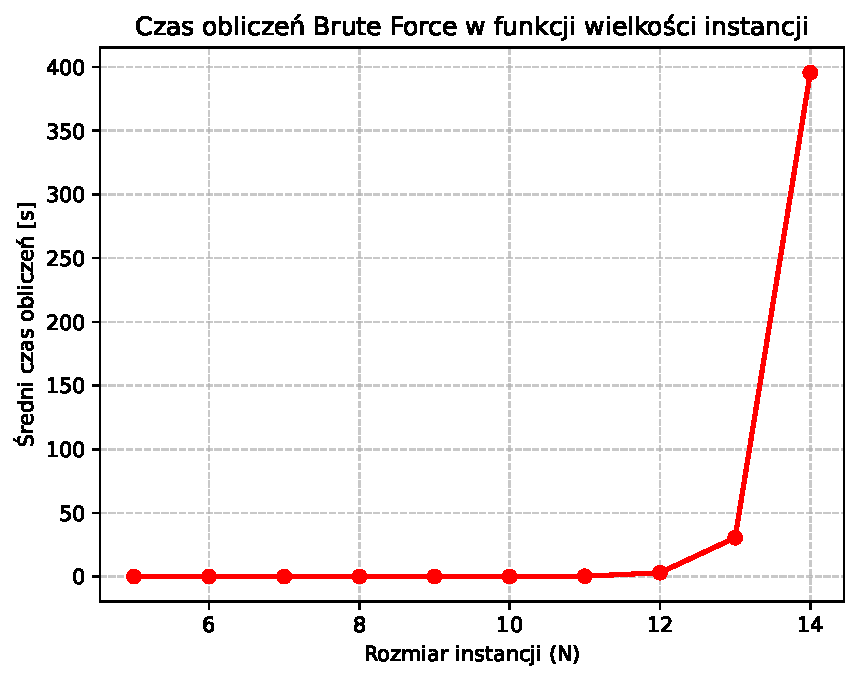
\includegraphics[width=0.8\textwidth]{rys/brute_force.pdf}
	\caption{Czas obliczeń algorytmu Brute-Force w funkcji rozmiaru instancji $N$.}
	\label{fig:bf_czas}
\end{figure}


Jak można zauważyć na powyższym wykresie, czas wykonania przeglądu zupełnego rośnie w sposób drastyczny. Potwierdza to teoretyczną złożoność $O(N!)$. Dla małych wartości $N$ (do 12) czas jest ułamkiem sekundy, jednak po przekroczeniu pewnego progu krzywa staje się niemal pionowa, co czyni ten algorytm nieużytecznym dla większych problemów. Dla rozmiaru instancji $N=15$ czas pomiaru przekroczył przyjętą granicę 30 minut. Zatem dla tego algorytmu górną granicą rozmiaru instancji jest $N=14$.
Uśrednione wyniki pomiarów przedstawiono w Tabeli \ref{tab:czasy_bf}.

Zupełnie inaczej prezentuje się charakterystyka algorytmów zachłannych (Nearest Neighbour oraz Repetitive Nearest Neighbour), co przedstawiono na Rysunku \ref{fig:nn_rnn_czas}. Wykres przedstawiono w skali logarytmicznej, więc zaprezentowany przebieg nie jest teoretycznym przebiegiem $N^3$ dla RNN oraz $N^2$ dla NN. Dla przyjętego ograniczenia czasu obliczeń na 10 minut, można przyjąć, że dla NN górną granicą instancji jest około $N=350~000$, zaś dla RNN $N=22~000$. Są to wartości daleko wykraczające poza możliwości algorytmu przeglądu zupełnego. 



\begin{table}[H]
	\centering
	\caption{Średni czas wykonania [s] dla algorytmu brute force w zależności od rozmiaru instancji $N$.}
	\label{tab:czasy_bf}
	\small
	\sisetup{
		exponent-mode = engineering, % Potęgi co 3
		round-mode = figures,
		round-precision = 4,
		output-decimal-marker = {,},
		exponent-product = \cdot
	} 
	\csvreader[
	separator=semicolon,
	no head,
	tabular={|c|c|},
	table head={\hline \textbf{N} & \textbf{Średni czas [s]} \\ \hline},
	late after line=\\\hline,
	filter test=\ifnumgreater{\thecsvinputline}{1}
	]{rys/bruteForce_time.csv}{1=\colN, 2=\colTime}{%
		\colN & \num{\colTime}
	}
\end{table}












\begin{figure}[H]
	\centering
	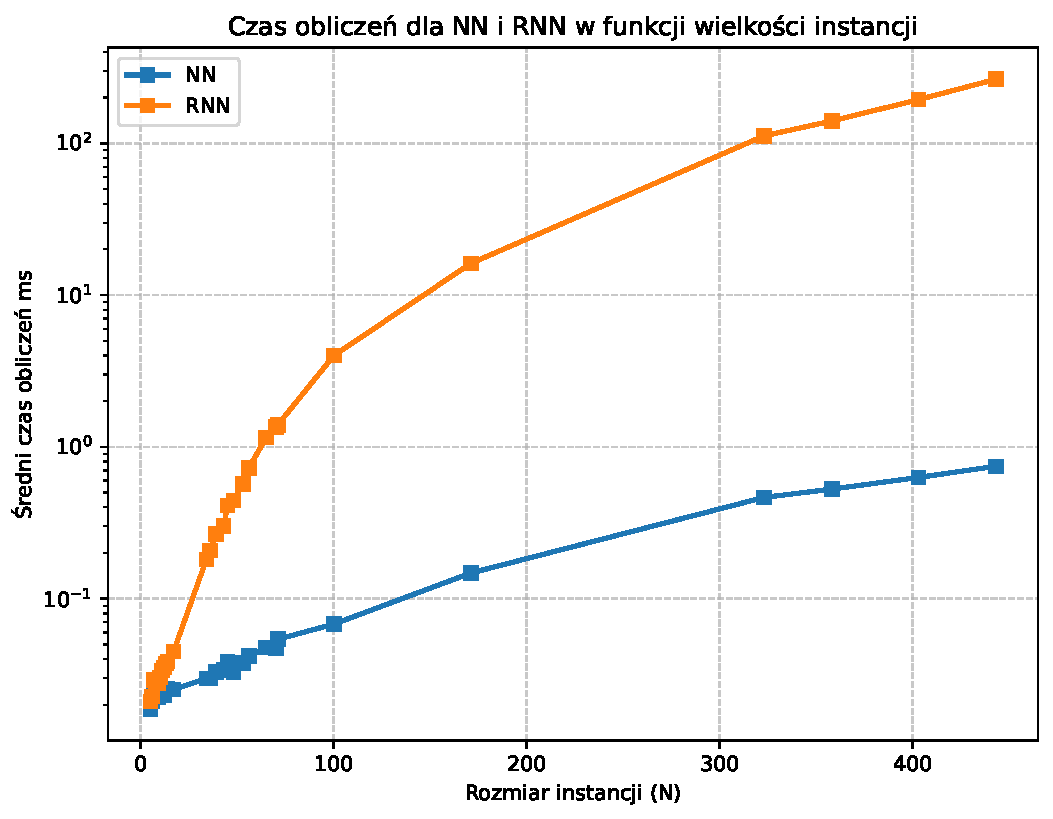
\includegraphics[width=0.8\textwidth]{rys/czas_nn_rnn_vs_n.pdf}
	\caption{Porównanie czasu obliczeń algorytmów heurystycznych NN i RNN.}
	\label{fig:nn_rnn_czas}
\end{figure}

Czasy wykonania obu heurystyk rosną wielomianowo, co pozwala na rozwiązywanie instancji o wiele większych niż w przypadku algorytmu dokładnego. Widać wyraźnie, że RNN, iterujący po każdym wierzchołku startowym, jest wolniejszy od klasycznego NN, jednak dla badanych wielkości $N \le 450$ czasy obu metod nadal pozostają na poziomie ułamków sekund. Szczegółowe wartości liczbowe dla algorytmów deterministycznych zebrano w Tabeli \ref{tab:wyniki_nn_rnn}. Czas wykonania RNN względem NN jest tyle razy większy ile wynosi rozmiar instancji, co wynika z faktu, że RNN to $N$ razy powtórzony NN ze zmienionym miastem startowym..

\begin{table}[H]
	\centering
	\caption{Dokładność i czas wykonania algorytmów NN i RNN (notacja inżynierska).}
	\label{tab:wyniki_nn_rnn}
	\small
	\sisetup{
		exponent-mode = engineering, % TO WYMUSZA POTĘGI CO 3
		round-mode = figures,
		round-precision = 4,
		output-decimal-marker = {,},
		exponent-product = \cdot
	} 
	\csvreader[
	separator=semicolon,
	no head,
	tabular={|c|c|c|c|c|},
	table head={\hline \textbf{N} & \textbf{Jakość NN [\%]} & \textbf{Jakość RNN [\%]} & \textbf{Czas NN [s]} & \textbf{Czas RNN [s]} \\ \hline},
	late after line=\\\hline,
	filter test=\ifnumgreater{\thecsvinputline}{1}
	]{rys/nn_rnn_time.csv}{1=\colN, 2=\colBNN, 3=\colBRNN, 4=\colTNN, 5=\colTRNN}{%
		\colN & 
		\num[exponent-mode=fixed]{\colBNN} & 
		\num[exponent-mode=fixed]{\colBRNN} & 
		\num{\colTNN} & 
		\num{\colTRNN}
	}
\end{table}


\subsection{Analiza dokładności algorytmów heurystycznych}

Kluczowym aspektem oceny heurystyk jest ich odchylenie od optymalnego kosztu trasy (błąd względny). Na Rysunku \ref{fig:nn_rnn_dokladnosc} zestawiono średnią dokładność algorytmów NN oraz RNN w funkcji rozmiaru instancji. Należy jednak mieć na uwadze, że sam błąd względny dla tych algorytmów jest zależny wyłącznie od danej instancji. Czyli dla różnych instancji w ramach tego samego rozmiaru instancji błąd względny będzie się zmieniał. Dla instancji generowanych losowo $N < 20$ błąd względny charakteryzuje się znacznym rozrzutem w porównaniu do instancji należących do TSPLIB. Jednakże, niezależnie od rozmiaru i instancji algorytm RNN będzie się charakteryzował mniejszym błędem niż NN. 

%Na Rysunku \ref{fig:nn_rnn_random_dokladnosc} zestawiono wyniki pomiarów dla NN i RNN z algorytmem losowym, przy czym czas pomiaru ograniczono do 1 sekundy. Jest to czas dwukrotnie większy, niż najdłuższy czas obliczeń dla RNN. W tym zakresie pomiarowym algorytmy NN i RNN są znacznie dokładniejsze.

\begin{figure}[H]
	\centering
	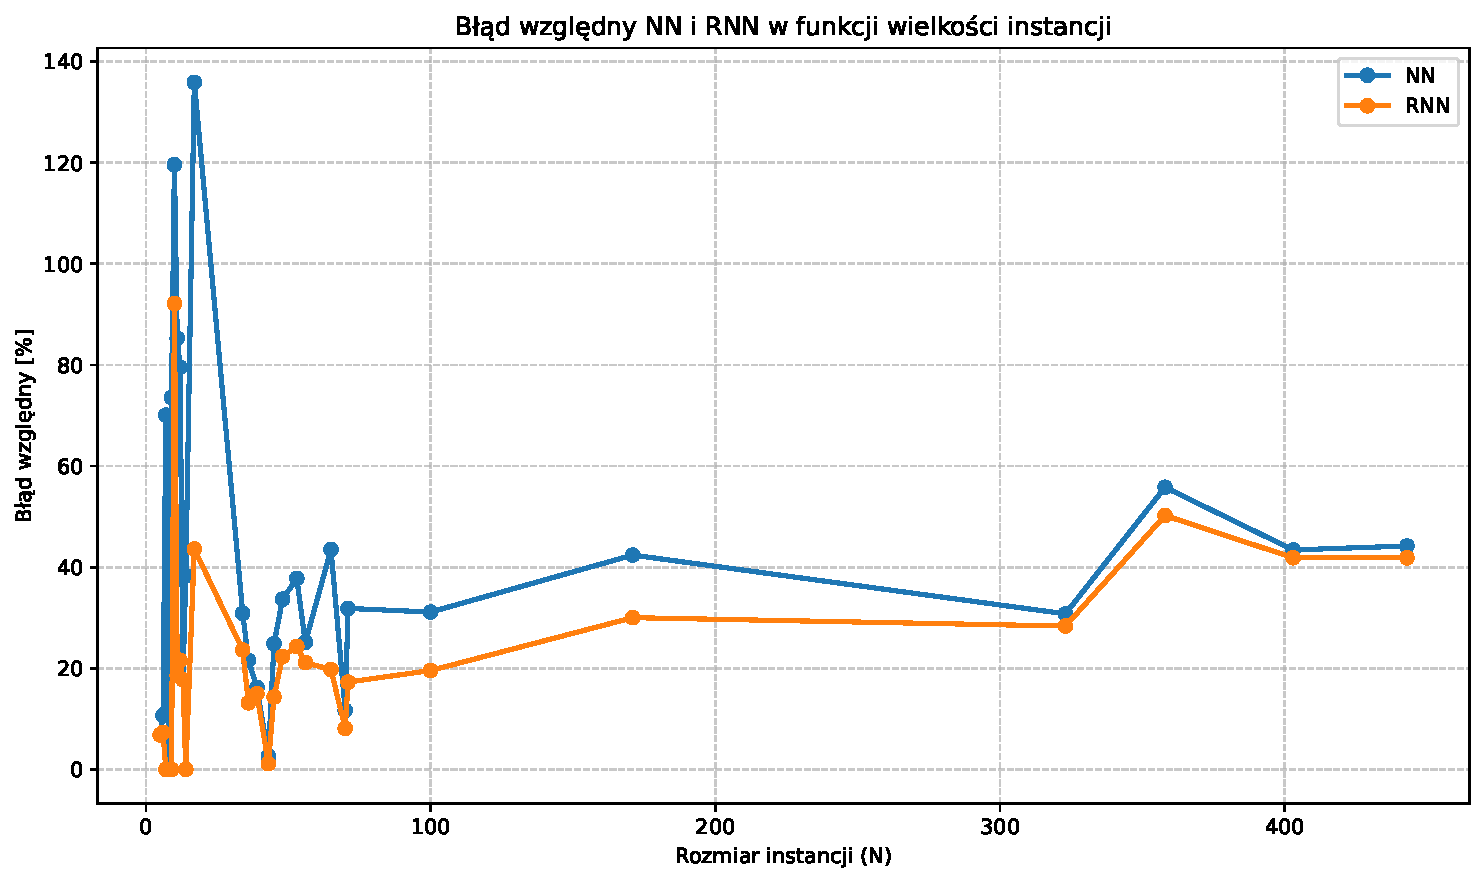
\includegraphics[width=0.8\textwidth]{rys/blad_nn_rnn_vs_n.pdf}
	\caption{Zależność czasu obliczeń od rozmiaru instancji dla NN i RNN.}
	\label{fig:nn_rnn_dokladnosc}
\end{figure}

%\begin{figure}[H]
%	\centering
%	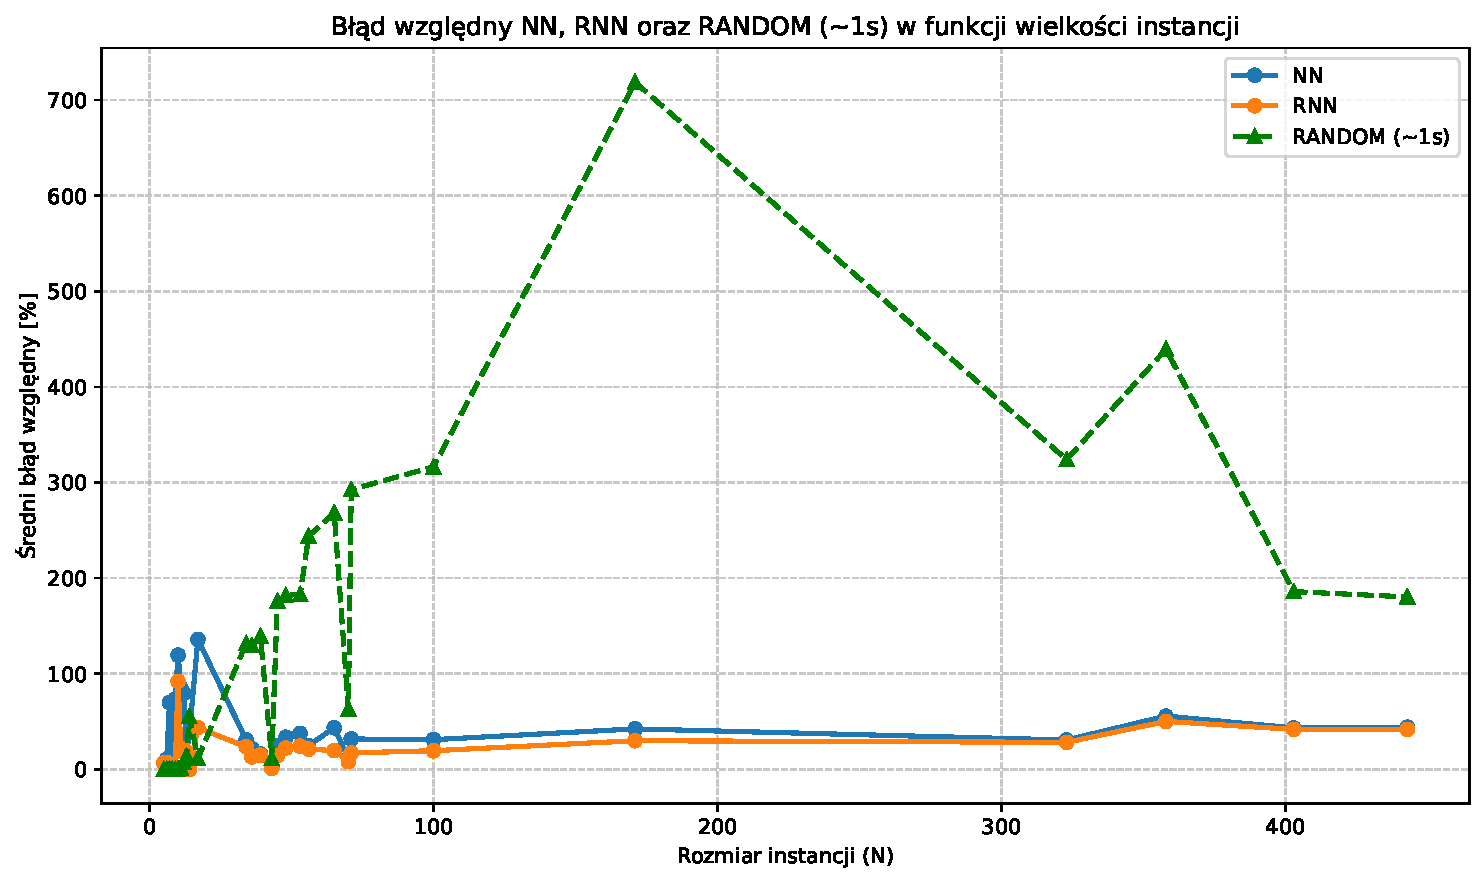
\includegraphics[width=0.8\textwidth]{rys/blad_nn_rnn_rand1s_vs_n.pdf}
%	\caption{Zależność czasu obliczeń od rozmiaru instancji dla NN i RNN.}
%	\label{fig:nn_rnn_rand_dokladnosc}
%\end{figure}


Wykres ten demonstruje wyższość algorytmu RNN nad NN -- kosztem dłuższego (ale wciąż akceptowalnego) czasu obliczeń, RNN oferuje znacznie wyższą i bardziej stabilną dokładność.





\subsection{Analiza rozrzutu algorytmu losowego}


Ze względu na stochastyczny charakter algorytmu losowego, poza średnim błędem względnym zbadano również rozrzut błędu względnego w zależności od czasu wykonywnia algorytmu. Na Rysunek \ref{fig:rand_rozrzut} przedstawiono wyniki pomiarowe dla wybranej instancji $N=14$.

Na poniższym wykresie można zobaczyć trend spadku średniego błędu względnego z około 50\% do około 20\% dla czasów pomiarowych wynoszących 55s-60s. Widać również ogromny rozrzut błędu średniego wynoszącym około 60\%. Analizując rozrzut można zauważyć, ze zdarzają sie przypadki pomiarowe, gdzie udało się trafić w optimum. Wynika to z faktu, że wykonano setki pomiarów w każdym przedziale pomiarowym, co w efekcie oznacza ponad 100-krotne zwiększenie czasu pomiarowego. 

Ponieważ do generowani losowego ciągu miast skorzystano z algorytmu Fischera, złożoność obliczeniowa wynosi $O(n)$ w efekcie pozwala to na wygenerowanie pojedynczego ciągu dla około miliona miast.



\begin{figure}[H]
	\centering
	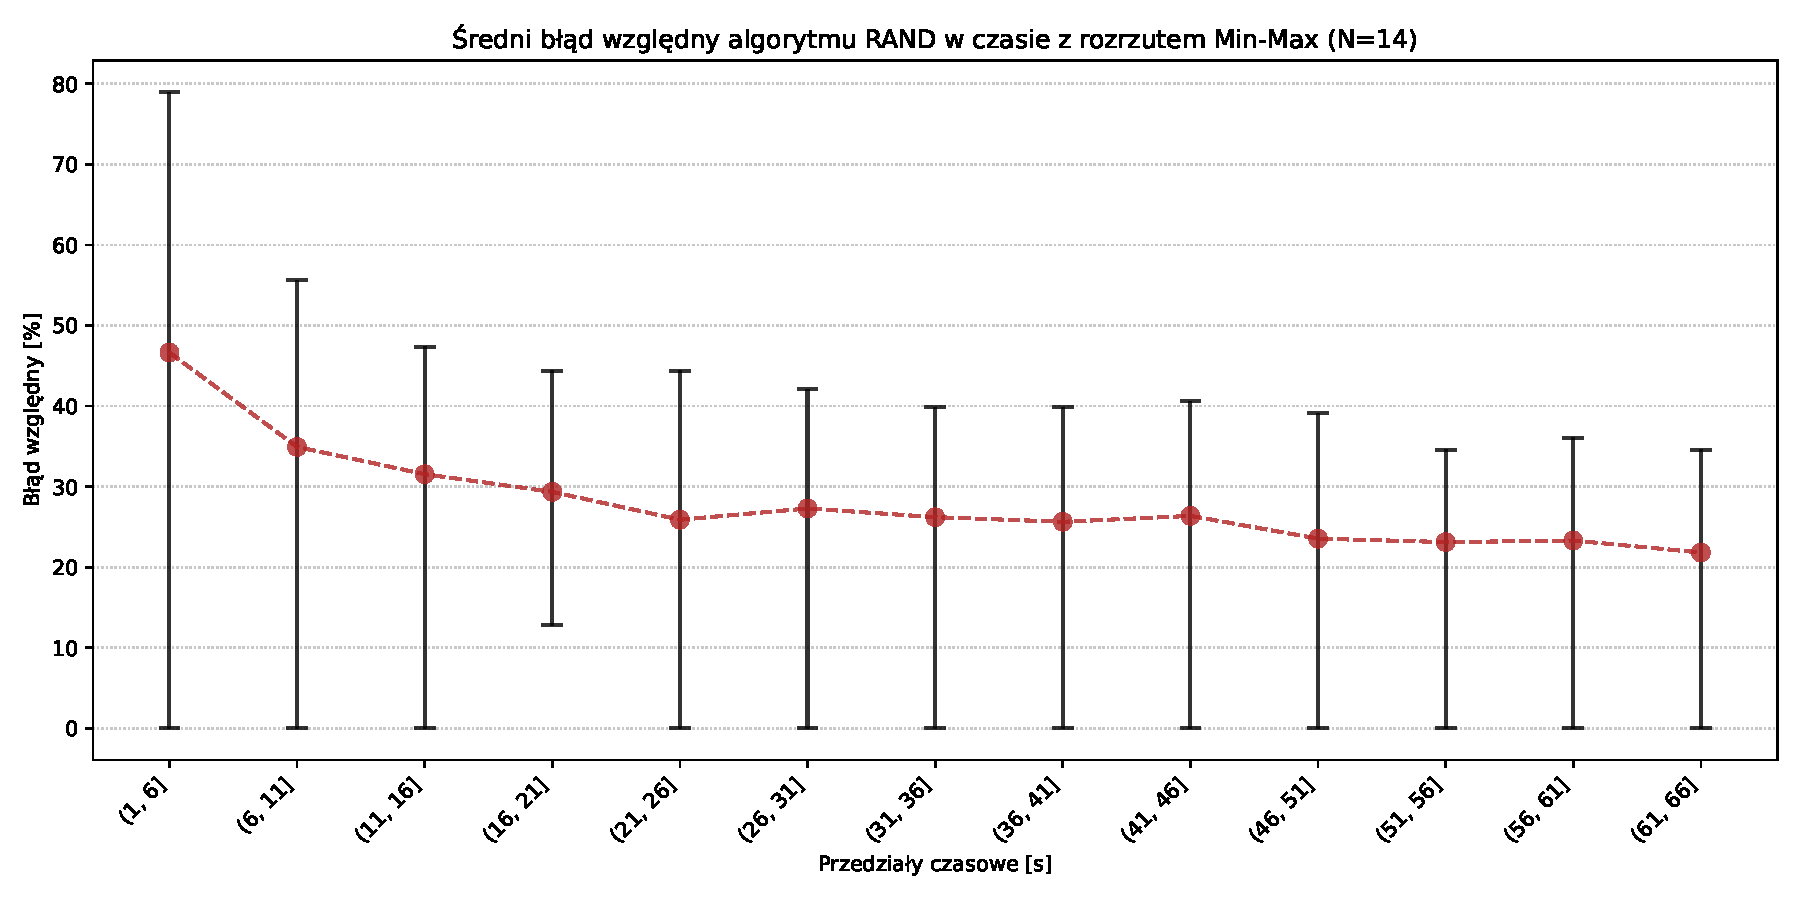
\includegraphics[width=0.8\textwidth]{rys/rand_errorbar_rozrzut.pdf}
	\caption{Zależność współcznnika jakości dla algorytmu losowego dla instancji $N=14$.}
	\label{fig:rand_rozrzut}
\end{figure}

\begin{figure}[H]
	\centering
	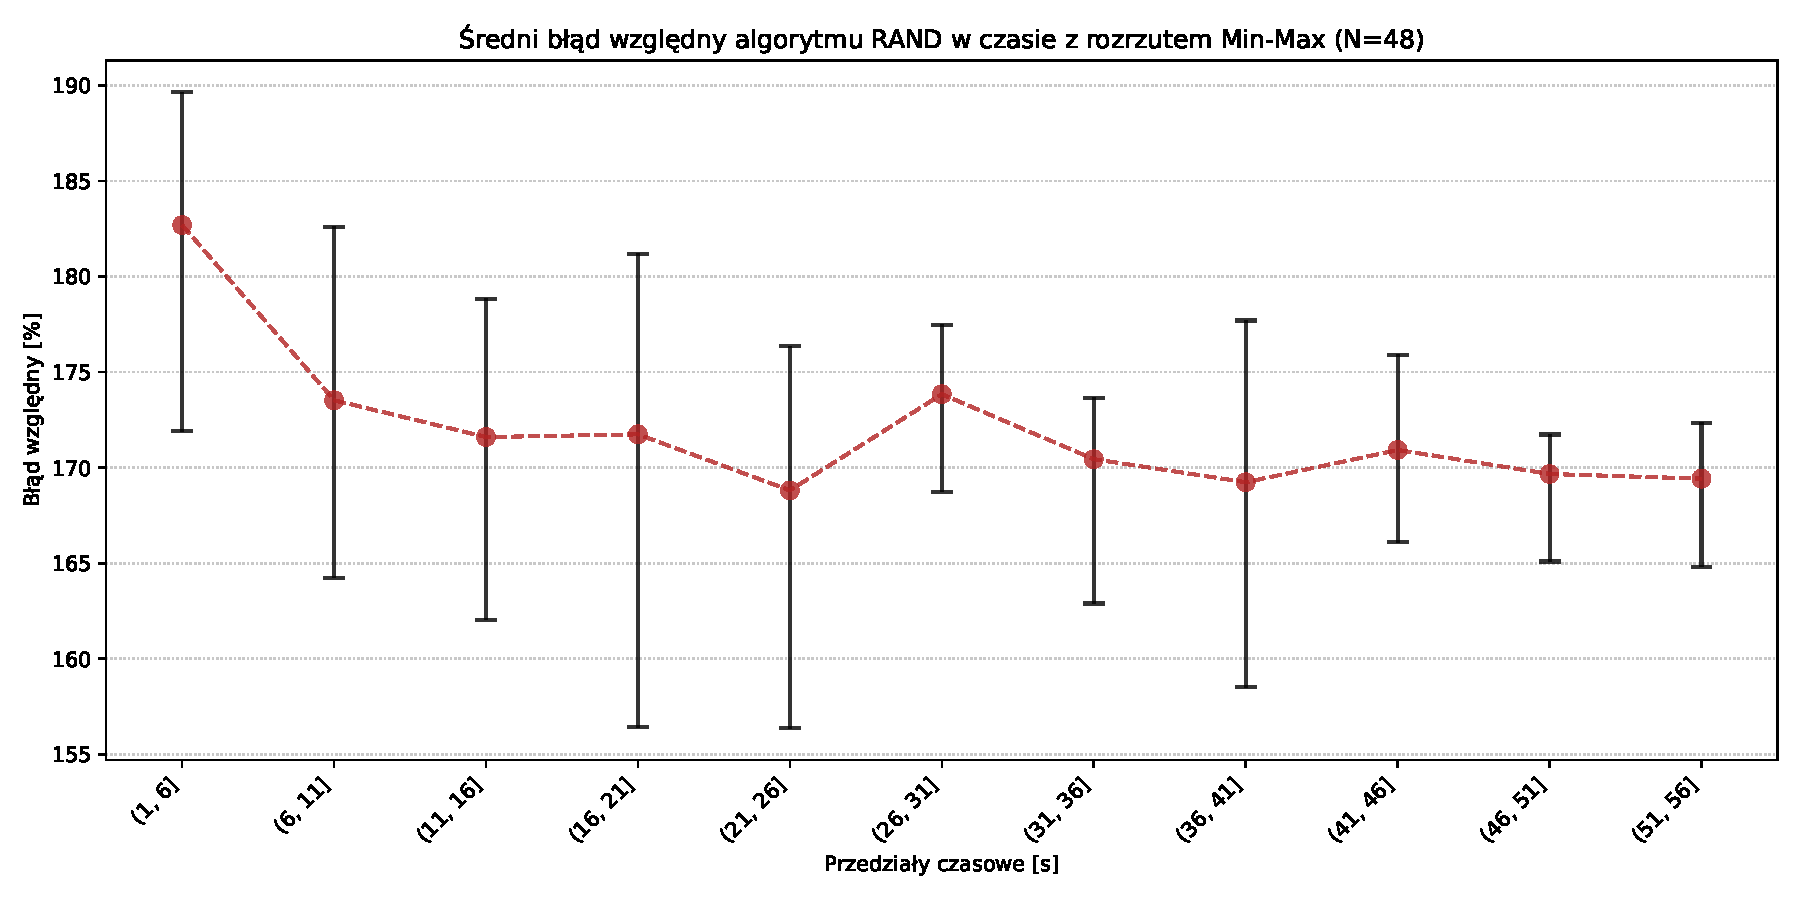
\includegraphics[width=0.8\textwidth]{rys/rand_errorbar_rozrzut_47.pdf}
	\caption{Zależność współcznnika jakości dla algorytmu losowego dla instancji $N=47$.}
	\label{fig:rand_rozrzut_47}
\end{figure}

\begin{figure}[H]
	\centering
	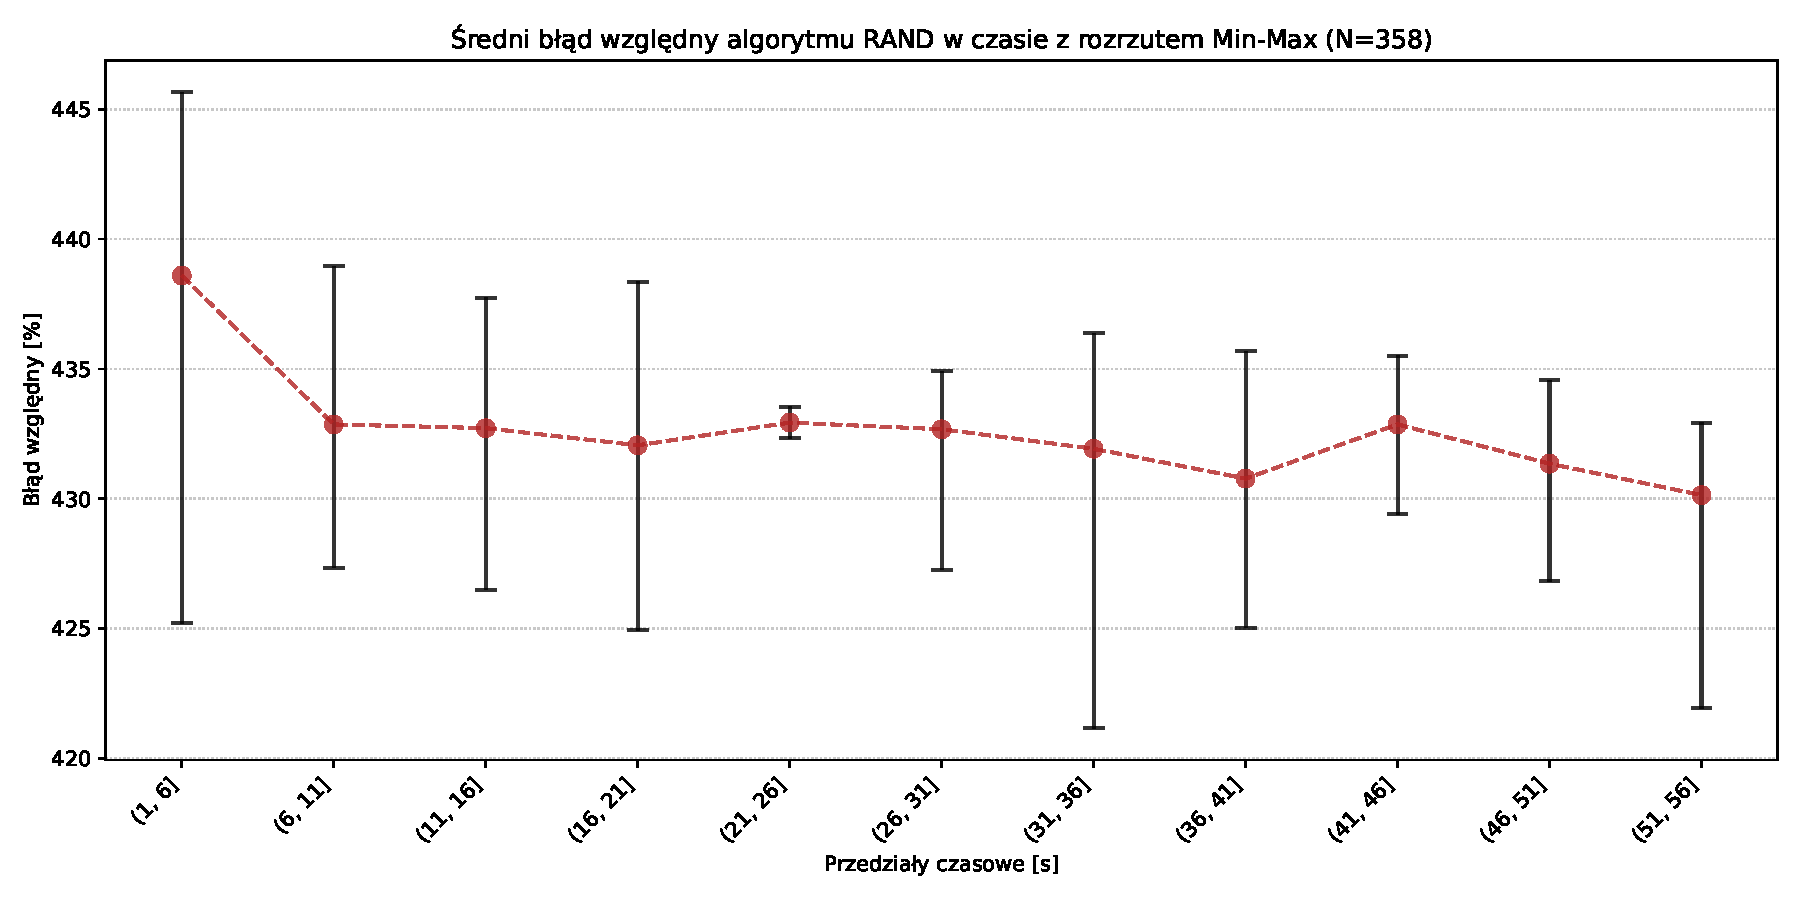
\includegraphics[width=0.8\textwidth]{rys/rand_errorbar_rozrzut_358.pdf}
	\caption{Zależność współcznnika jakości dla algorytmu losowego dla instancji $N=358$.}
	\label{fig:rand_rozrzut_358}
\end{figure}


\section{Podsumowanie i wnioski}

Przeprowadzone eksperymenty oraz implementacja algorytmów dla Asymetrycznego Problemu Komiwojażera pozwalają na sformułowanie następujących wniosków końcowych:

\begin{enumerate}
	\item \textbf{Ograniczenia przeglądu zupełnego:} Algorytm Brute-Force, choć gwarantuje znalezienie absolutnego optimum, jest użyteczny wyłącznie dla najmniejszych instancji (do $N \approx 14$). Złożoność silniowa $O(N!)$ sprawia, że dołożenie choćby jednego miasta do grafu drastycznie (kilkunastokrotnie) wydłuża czas oczekiwania, deklasując tę metodę w zastosowaniach praktycznych.
	
	\item \textbf{Pułapki lokalne algorytmu Nearest Neighbour:} Zwykły algorytm najbliższego sąsiada (NN) wykazuje się znakomitym czasem wykonania $O(N^2)$. Jest w stanie obsłużyć potężne grafy w ułamku sekundy. Niestety, jego czysto zachłanna natura powoduje, że pod koniec wyznaczania trasy zmuszony jest do wyboru bardzo kosztownych krawędzi. Czyni to wygenerowane rozwiązanie dalekim od optimum. Maksymalny rozmiar instancji $N \approx 350~000$.
	
	\item \textbf{Kompromis Repetitive Nearest Neighbour:} Zastosowanie nakładki w postaci uruchamiania metody zachłannej z każdego możliwego wierzchołka startowego (RNN) okazało się w tym eksperymencie najbardziej racjonalnym kompromisem. Czas działania $O(N^3)$ wciąż pozwala na błyskawiczne rozwiązywanie problemu w czasie wielomianowym, a wyeliminowanie zjawiska ,,złego miasta startowego'' znacząco podnosi dokładność rozwiązania. Maksymalny rozmiar instancji $N \approx 22~000$
	
	\item \textbf{Nieefektywność ślepego losowania:} Metoda losowa stanowi dobre tło porównawcze (baseline), jednak nie posiada żadnej wartości aplikacyjnej. W grafach rzędu $N > 10$ znalezienie w pełni optymalnej ścieżki wymagałoby niewyobrażalnego czasu. Co prawda, dokładność rośnie wraz z zadanym limitem czasu (co widać w analizie makro), jednak ten sam efekt algorytm RNN osiąga tysiące razy szybciej w sposób deterministyczny. Maksymalny rozmiar instancji $N \approx 1 000 000$ (bez gwarancji sensownego wyniku).
\end{enumerate}

Podsumowując, do rozwiązywania problemów klasy ATSP na dużą skalę w rzeczywistych warunkach niezbędne jest odrzucenie metod dokładnych na rzecz zaawansowanych algorytmów przybliżonych (np. metaheurystyk), których wstępną bazę może stanowić algorytm oparty na zasadzie Repetitive Nearest Neighbour.	
	

\newpage

\section{Środowisko testowe}
W celu zapewnienia powtarzalności wyników oraz rzetelnej analizy wydajności zaimplementowanych algorytmów, wszystkie testy zostały przeprowadzone w ustandaryzowanym środowisku sprzętowo-programowym. Specyfikacja techniczna jednostki obliczeniowej została przedstawiona poniżej:

\subsection{Specyfikacja sprzętowa}
\begin{itemize}
	\item \textbf{Procesor:} AMD Ryzen 7 5800H (8 rdzeni, 16 wątków). Architektura Zen 3 (Cezanne).
	\item \textbf{Pamięć Cache:}
	\begin{itemize}
		\item L1 cache: 512 KiB
		\item L2 cache: 4 MiB
		\item L3 cache: 16 MiB (współdzielona)
	\end{itemize}
	\item \textbf{Pamięć RAM:} 16 GiB DDR4 Synchronous (2 x 8 GiB, praca w trybie Dual-Channel).
	\item \textbf{Dysk:} NVMe SSD Samsung 1024 GB (wykorzystywany do zapisu logów i wyników CSV).
	\item \textbf{Karta graficzna:} NVIDIA GeForce GTX 1650 Mobile / AMD Radeon Vega Series (nieużywane w procesie obliczeń CPU-bound).
\end{itemize}

\subsection{Środowisko programowe}
\begin{itemize}
	\item \textbf{System operacyjny:} Linux (Ubuntu) 
	\item \textbf{Język programowania:} C++23 (Standard ISO/IEC 14882:2023)
	\item \textbf{Kompilator:} GCC/G++ (wykorzystujący optymalizacje poziomu \texttt{-O3})
	\item \textbf{Narzędzia analityczne:} Python 3.x (biblioteki Pandas, Matplotlib) do generowania wykresów i analizy statystycznej.
\end{itemize}


	
	
\end{document}